\documentclass[11pt,preprint, authoryear]{elsarticle}

\usepackage{lmodern}
%%%% My spacing
\usepackage{setspace}
\setstretch{1.2}
\DeclareMathSizes{12}{14}{10}{10}

% Wrap around which gives all figures included the [H] command, or places it "here". This can be tedious to code in Rmarkdown.
\usepackage{float}
\let\origfigure\figure
\let\endorigfigure\endfigure
\renewenvironment{figure}[1][2] {
    \expandafter\origfigure\expandafter[H]
} {
    \endorigfigure
}

\let\origtable\table
\let\endorigtable\endtable
\renewenvironment{table}[1][2] {
    \expandafter\origtable\expandafter[H]
} {
    \endorigtable
}


\usepackage{ifxetex,ifluatex}
\usepackage{fixltx2e} % provides \textsubscript
\ifnum 0\ifxetex 1\fi\ifluatex 1\fi=0 % if pdftex
  \usepackage[T1]{fontenc}
  \usepackage[utf8]{inputenc}
\else % if luatex or xelatex
  \ifxetex
    \usepackage{mathspec}
    \usepackage{xltxtra,xunicode}
  \else
    \usepackage{fontspec}
  \fi
  \defaultfontfeatures{Mapping=tex-text,Scale=MatchLowercase}
  \newcommand{\euro}{€}
\fi

\usepackage{amssymb, amsmath, amsthm, amsfonts}

\def\bibsection{\section*{References}} %%% Make "References" appear before bibliography


\usepackage[round]{natbib}

\usepackage{longtable}
\usepackage[margin=2.3cm,bottom=2cm,top=2.5cm, includefoot]{geometry}
\usepackage{fancyhdr}
\usepackage[bottom, hang, flushmargin]{footmisc}
\usepackage{graphicx}
\numberwithin{equation}{section}
\numberwithin{figure}{section}
\numberwithin{table}{section}
\setlength{\parindent}{0cm}
\setlength{\parskip}{1.3ex plus 0.5ex minus 0.3ex}
\usepackage{textcomp}
\renewcommand{\headrulewidth}{0pt}

\usepackage{array}
\newcolumntype{x}[1]{>{\centering\arraybackslash\hspace{0pt}}p{#1}}

%%%%  Remove the "preprint submitted to" part. Don't worry about this either, it just looks better without it:
\makeatletter
\def\ps@pprintTitle{%
  \let\@oddhead\@empty
  \let\@evenhead\@empty
  \let\@oddfoot\@empty
  \let\@evenfoot\@oddfoot
}
\makeatother

 \def\tightlist{} % This allows for subbullets!

\usepackage{hyperref}
\hypersetup{breaklinks=true,
            bookmarks=true,
            colorlinks=true,
            citecolor=blue,
            urlcolor=blue,
            linkcolor=blue,
            pdfborder={0 0 0}}


% The following packages allow huxtable to work:
\usepackage{siunitx}
\usepackage{multirow}
\usepackage{hhline}
\usepackage{calc}
\usepackage{tabularx}
\usepackage{booktabs}
\usepackage{caption}


\newenvironment{columns}[1][]{}{}

\newenvironment{column}[1]{\begin{minipage}{#1}\ignorespaces}{%
\end{minipage}
\ifhmode\unskip\fi
\aftergroup\useignorespacesandallpars}

\def\useignorespacesandallpars#1\ignorespaces\fi{%
#1\fi\ignorespacesandallpars}

\makeatletter
\def\ignorespacesandallpars{%
  \@ifnextchar\par
    {\expandafter\ignorespacesandallpars\@gobble}%
    {}%
}
\makeatother

\newlength{\cslhangindent}
\setlength{\cslhangindent}{1.5em}
\newenvironment{CSLReferences}%
  {\setlength{\parindent}{0pt}%
  \everypar{\setlength{\hangindent}{\cslhangindent}}\ignorespaces}%
  {\par}


\urlstyle{same}  % don't use monospace font for urls
\setlength{\parindent}{0pt}
\setlength{\parskip}{6pt plus 2pt minus 1pt}
\setlength{\emergencystretch}{3em}  % prevent overfull lines
\setcounter{secnumdepth}{5}

%%% Use protect on footnotes to avoid problems with footnotes in titles
\let\rmarkdownfootnote\footnote%
\def\footnote{\protect\rmarkdownfootnote}
\IfFileExists{upquote.sty}{\usepackage{upquote}}{}

%%% Include extra packages specified by user
\usepackage{booktabs}
\usepackage{longtable}
\usepackage{array}
\usepackage{multirow}
\usepackage{wrapfig}
\usepackage{float}
\usepackage{colortbl}
\usepackage{pdflscape}
\usepackage{tabu}
\usepackage{threeparttable}
\usepackage{threeparttablex}
\usepackage[normalem]{ulem}
\usepackage{makecell}
\usepackage{xcolor}

%%% Hard setting column skips for reports - this ensures greater consistency and control over the length settings in the document.
%% page layout
%% paragraphs
\setlength{\baselineskip}{12pt plus 0pt minus 0pt}
\setlength{\parskip}{12pt plus 0pt minus 0pt}
\setlength{\parindent}{0pt plus 0pt minus 0pt}
%% floats
\setlength{\floatsep}{12pt plus 0 pt minus 0pt}
\setlength{\textfloatsep}{20pt plus 0pt minus 0pt}
\setlength{\intextsep}{14pt plus 0pt minus 0pt}
\setlength{\dbltextfloatsep}{20pt plus 0pt minus 0pt}
\setlength{\dblfloatsep}{14pt plus 0pt minus 0pt}
%% maths
\setlength{\abovedisplayskip}{12pt plus 0pt minus 0pt}
\setlength{\belowdisplayskip}{12pt plus 0pt minus 0pt}
%% lists
\setlength{\topsep}{10pt plus 0pt minus 0pt}
\setlength{\partopsep}{3pt plus 0pt minus 0pt}
\setlength{\itemsep}{5pt plus 0pt minus 0pt}
\setlength{\labelsep}{8mm plus 0mm minus 0mm}
\setlength{\parsep}{\the\parskip}
\setlength{\listparindent}{\the\parindent}
%% verbatim
\setlength{\fboxsep}{5pt plus 0pt minus 0pt}



\begin{document}



\begin{frontmatter}  %

\title{Comparing SVR to LSTM ANN for Volatility Forecasting}

% Set to FALSE if wanting to remove title (for submission)




\author[Add1]{Jonathan Rossouw}
\ead{20858345@sun.ac.za}







\begin{abstract}
\small{
Volatility modelling is an important problem in financial econmetrics.
The recent prolierfation of powerful machine learning techniques offers
a models that are well suited to this complex problem. In this paper
volatility forecasting by Support Vector Regression (SVR) and Long-Short
Term Memory Recurrent Neural Networks (LSTM) are compared. The JSE All
Share index is used to compare. An EGARCH models is used as a baseline
model. The LSTM model performed best at one-day ahead and three-day
ahead forecasting.
}
\end{abstract}

\vspace{1cm}





\vspace{0.5cm}

\end{frontmatter}



%________________________
% Header and Footers
%%%%%%%%%%%%%%%%%%%%%%%%%%%%%%%%%
\pagestyle{fancy}
\chead{}
\rhead{}
\lfoot{}
\rfoot{}
\lhead{}
%\rfoot{\footnotesize Page \thepage } % "e.g. Page 2"
\cfoot{}

%\setlength\headheight{30pt}
%%%%%%%%%%%%%%%%%%%%%%%%%%%%%%%%%
%________________________

\headsep 35pt % So that header does not go over title




\hypertarget{introduction}{%
\section{\texorpdfstring{Introduction
\label{Introduction}}{Introduction }}\label{introduction}}

Volatility modelling is an important and complex problem in financial
econometrics. The volatility the returns of an asset are an important
measure for the risk of an asset. Volatility itself is a key factor in
options pricing and in asset allocation. The Value-at-Risk calculations
made for risk management rely on measures of volatility. There has been
a recent proliferation of machine learning techniques that can greatly
improve the precision of volatility forecasting. The traditional
forecasting techniques build on the generalized autoregressive
conditional heteroscedastic (GARCH) class of models are well suited for
uncovering the true patterns of volatility. However, their ability to
accurately forecast volatility is limited.

\par

The use of machine learning techniques including Support Vector
Regression (SVR) and artifical neural network models has grown in recent
years with far superior performance (citation needed). Recently proposed
volatility models using the long-short term memeroy recurrent neural
network (LSTM) have futher improved forecasting precision(citation
needed). While these models have been used to model volatility in the
US, only the SVR and GARCH models have been applied to South African
data.

\par

The volatility of the JSE ALSI total returns index (TRI) is modelled.
This paper finds that the GARCH models perform poorly on pure
forecasting precision. The SVR and LSTM models perform similarly well on
one-day ahead forecasting with the LSTM marginally better. On three-day
ahead forecasting

The remainder of the paper is organised as follows: the data and
methodology is described, the results are analysed followed by the
conclusion.

\hypertarget{data}{%
\section*{Data}\label{data}}
\addcontentsline{toc}{section}{Data}

The data used in this paper is the total return index (TRI) of the JSE
ALSI. The TRI is price adjusted for dividends, stock splits and other
corporate actions. The data is split into training, validation and test
series. The training set is from 05-01-2009 to 30-12-2016, the
validation set is from 03-01-2017 to 31-12-2018, and the test set is
from 03-01-2019 to 31-12-2019. Returns, dlogret, are calculated using
log difference of TRI, log(TRI) - log(lag(TRI)). The volatility, sigma,
is calculated as dlogret\^{}2.

\hypertarget{methodology}{%
\section{\texorpdfstring{Methodology
\label{Meth}}{Methodology }}\label{methodology}}

\hypertarget{results}{%
\section{Results}\label{results}}

\begin{verbatim}
## $`Return Plots`
\end{verbatim}

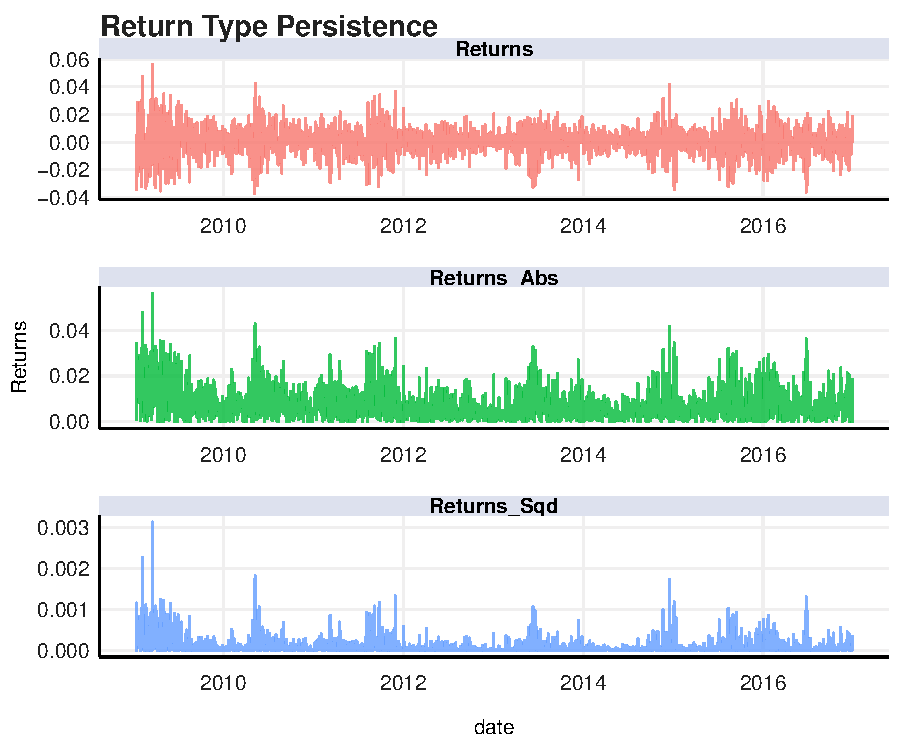
\includegraphics{Essay_files/figure-latex/garch-1.pdf}

\begin{verbatim}
## 
## $`ACF Plots`
\end{verbatim}

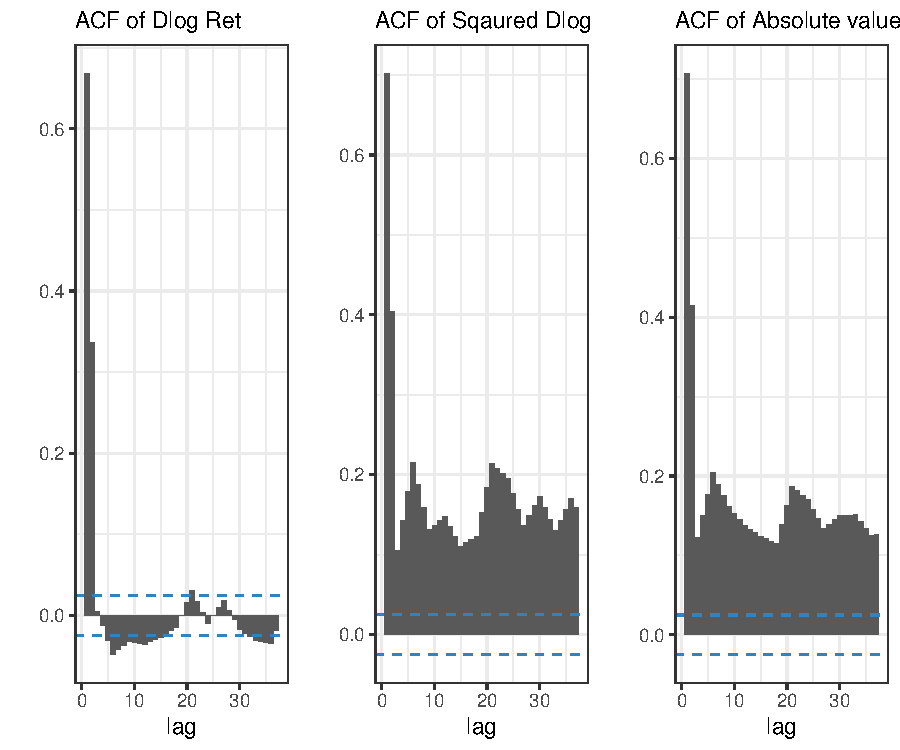
\includegraphics{Essay_files/figure-latex/garch-2.pdf}

\begin{verbatim}
## 
## $`Box Statistics`
## 
##  Box-Ljung test
## 
## data:  data$dlogret^2
## X-squared = 632.57, df = 12, p-value < 2.2e-16
\end{verbatim}

\begin{verbatim}
##                 sGARCH  gjrGARCH    eGARCH    apARCH
## Akaike       -6.452107 -6.482330 -6.490124 -6.476212
## Bayes        -6.438554 -6.466067 -6.473860 -6.457238
## Shibata      -6.452119 -6.482347 -6.490140 -6.476235
## Hannan-Quinn -6.447141 -6.476371 -6.484164 -6.469259
\end{verbatim}

\begin{verbatim}
##             Estimate   Std. Error       t value     Pr(>|t|)
## mu      0.0003515747 2.130849e-04     1.6499274 9.895778e-02
## ar1     0.0125580135 3.000059e-02     0.4185922 6.755142e-01
## omega  -0.1158799416 3.678887e-03   -31.4986395 0.000000e+00
## alpha1 -0.1229697781 1.276882e-02    -9.6304719 0.000000e+00
## beta1   0.9876109595 3.831107e-05 25778.7351700 0.000000e+00
## gamma1  0.0827979223 8.778569e-03     9.4318240 0.000000e+00
## shape  11.8303799861 2.471258e+00     4.7871886 1.691339e-06
\end{verbatim}

\begin{verbatim}
##             Estimate   Std. Error      t value     Pr(>|t|)
## mu      0.0002864073 0.0003012782    0.9506407 3.417868e-01
## ar1     0.0264570892 0.0442049551    0.5985096 5.495000e-01
## omega  -0.3238038491 0.0070088366  -46.1993718 0.000000e+00
## alpha1 -0.1486355485 0.0223898006   -6.6385383 3.168088e-11
## beta1   0.9667674863 0.0001089335 8874.8383943 0.000000e+00
## gamma1  0.0614327405 0.0272134808    2.2574378 2.398073e-02
## shape   8.2762798876 2.8918533902    2.8619293 4.210709e-03
\end{verbatim}

\begin{verbatim}
## [1] 0.003458062
\end{verbatim}

\begin{verbatim}
## [1] 0.009582018
\end{verbatim}

\begin{figure}[H]

{\centering 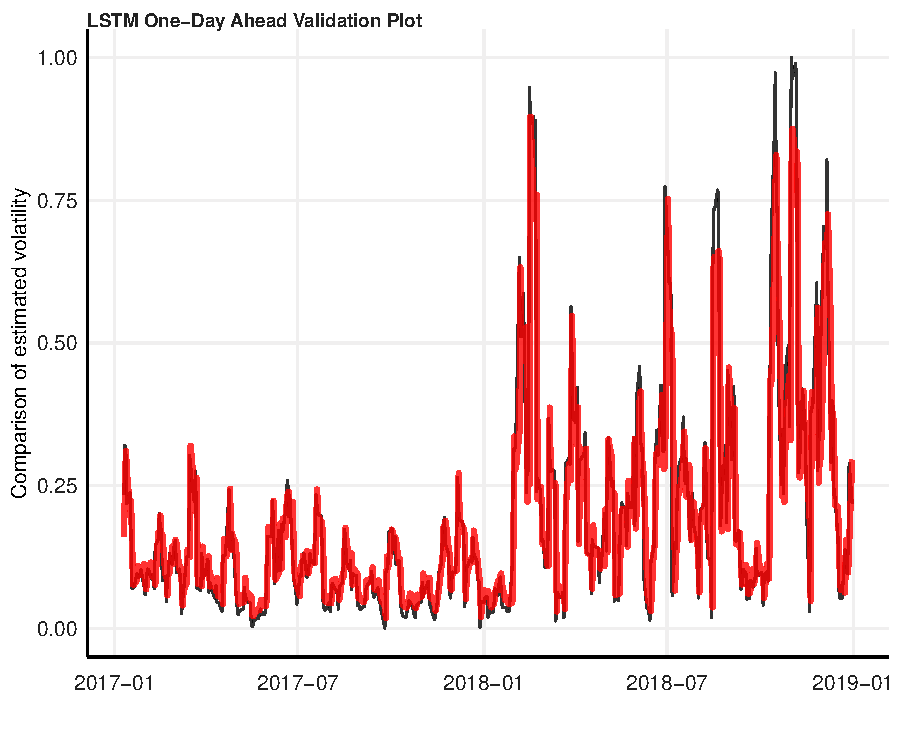
\includegraphics{Essay_files/figure-latex/plot_val-1} 

}

\caption{LSTM One-Day Ahead Validation Forecast}\label{fig:plot_val}
\end{figure}

\begin{verbatim}
## [1] 0.01517164
\end{verbatim}

\begin{verbatim}
## [1] 0.04770794
\end{verbatim}

\begin{verbatim}
## [1] "1 DONE!!"
## [1] "DONE!!"
\end{verbatim}

\begin{verbatim}
## # A tibble: 1 x 3
##    gamma lambda     mse
##    <dbl>  <dbl>   <dbl>
## 1 0.0821 0.0821 0.00342
\end{verbatim}

\begin{verbatim}
## # A tibble: 1 x 3
##    gamma lambda     mse
##    <dbl>  <dbl>   <dbl>
## 1 0.0821 0.0821 0.00968
\end{verbatim}

\begin{verbatim}
## [1] "1 DONE!!"
## [1] "DONE!!"
\end{verbatim}

\begin{verbatim}
## # A tibble: 1 x 3
##    gamma lambda     mse
##    <dbl>  <dbl>   <dbl>
## 1 0.0821 0.0821 0.00813
\end{verbatim}

\begin{verbatim}
## # A tibble: 1 x 3
##    gamma lambda    mse
##    <dbl>  <dbl>  <dbl>
## 1 0.0821 0.0821 0.0462
\end{verbatim}

\begin{figure}[H]

{\centering 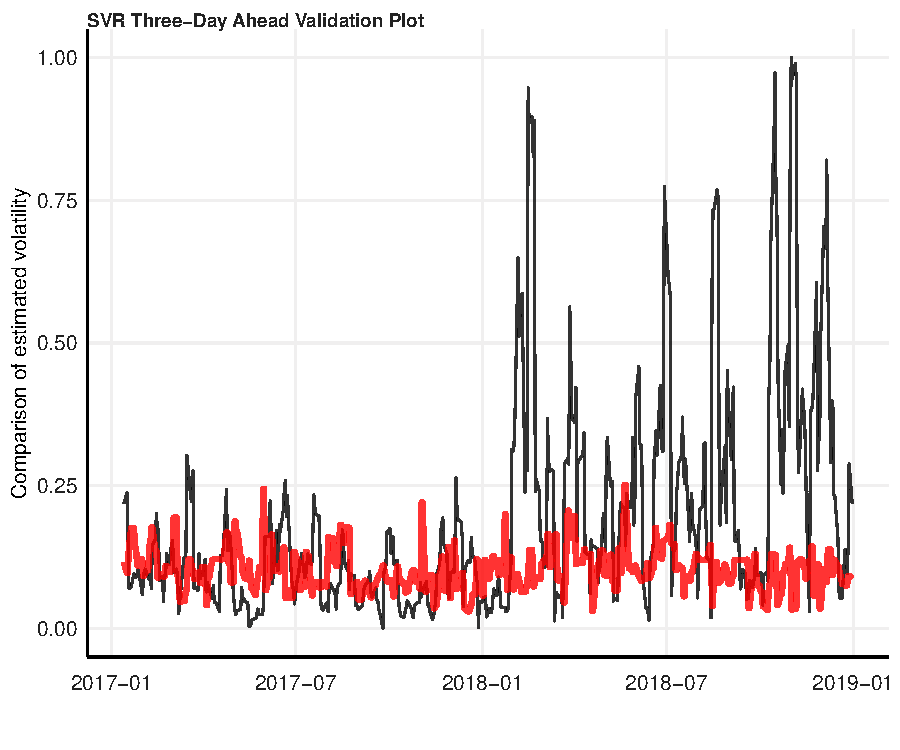
\includegraphics{Essay_files/figure-latex/plot_val_3-1} 

}

\caption{SVR Three-Day Ahead Validation Forecast}\label{fig:plot_val_3}
\end{figure}

\begin{verbatim}
## [1] 0.003129262
\end{verbatim}

\begin{verbatim}
## [1] 0.01206342
\end{verbatim}

\begin{figure}[H]

{\centering 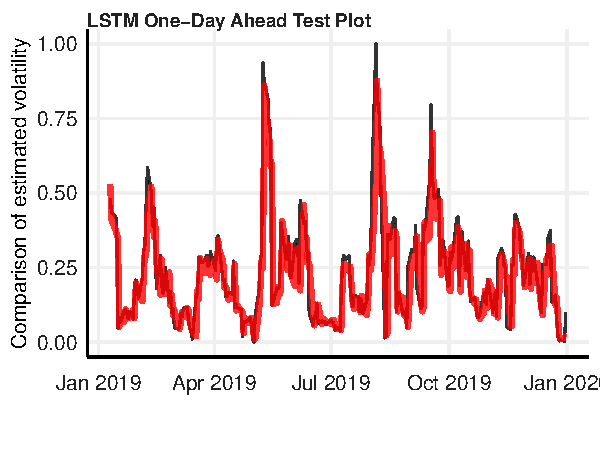
\includegraphics{Essay_files/figure-latex/plot_test-1} 

}

\caption{LSTM One-Day Ahead Test Forecast}\label{fig:plot_test}
\end{figure}

\begin{verbatim}
## [1] "1 DONE!!"
## [1] "DONE!!"
\end{verbatim}

\begin{verbatim}
## # A tibble: 1 x 3
##    gamma lambda     mse
##    <dbl>  <dbl>   <dbl>
## 1 0.0821 0.0821 0.00372
\end{verbatim}

\begin{verbatim}
## # A tibble: 1 x 3
##    gamma lambda    mse
##    <dbl>  <dbl>  <dbl>
## 1 0.0821 0.0821 0.0523
\end{verbatim}

\begin{figure}[H]

{\centering 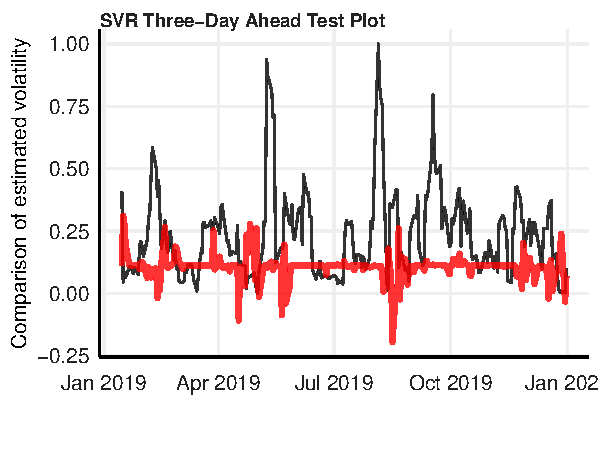
\includegraphics{Essay_files/figure-latex/plot_3_test-1} 

}

\caption{LSTM Three-Day Ahead Test Forecast}\label{fig:plot_3_test}
\end{figure}

\hypertarget{conclusion}{%
\section{Conclusion}\label{conclusion}}

\newpage

\hypertarget{references}{%
\section*{References}\label{references}}
\addcontentsline{toc}{section}{References}

\hypertarget{refs}{}
\begin{CSLReferences}{0}{0}
\end{CSLReferences}

\hypertarget{appendix}{%
\section*{Appendix}\label{appendix}}
\addcontentsline{toc}{section}{Appendix}

\begin{figure}[H]

{\centering 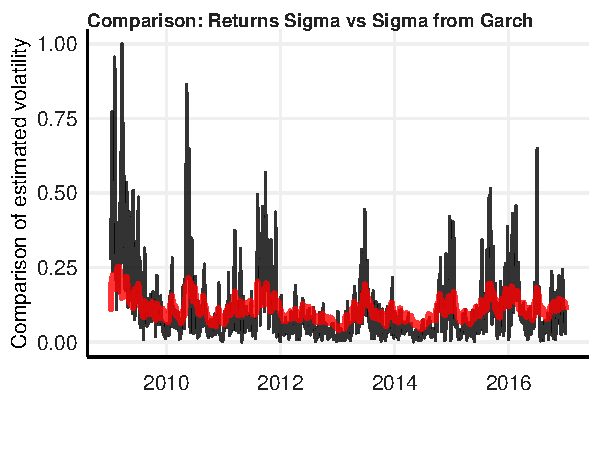
\includegraphics{Essay_files/figure-latex/plot_1-1} 

}

\caption{EGARCH(1,1) One-Day Ahead Training Forecast}\label{fig:plot_1}
\end{figure}

\begin{figure}[H]

{\centering 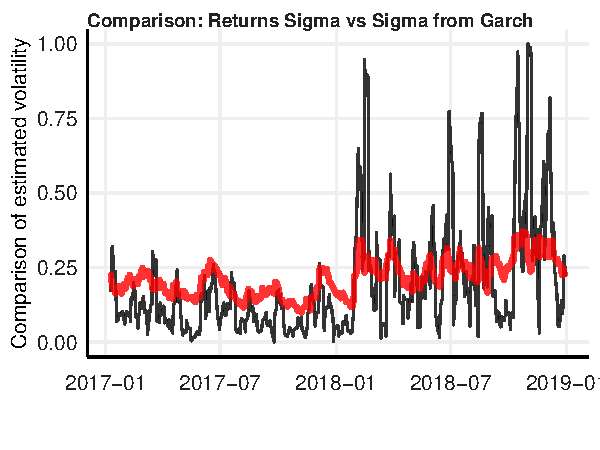
\includegraphics{Essay_files/figure-latex/plot_2-1} 

}

\caption{EGARCH(1,1) One-Day Ahead Validation Forecast}\label{fig:plot_2}
\end{figure}

\begin{figure}[H]

{\centering 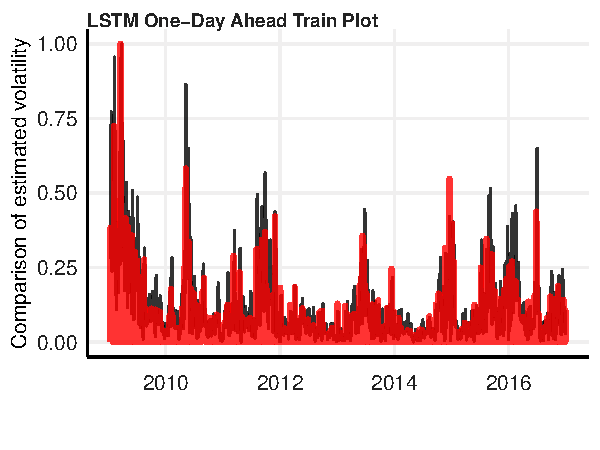
\includegraphics{Essay_files/figure-latex/plot_3-1} 

}

\caption{LSTM One-Day Ahead Training Forecast}\label{fig:plot_3}
\end{figure}

\begin{figure}[H]

{\centering 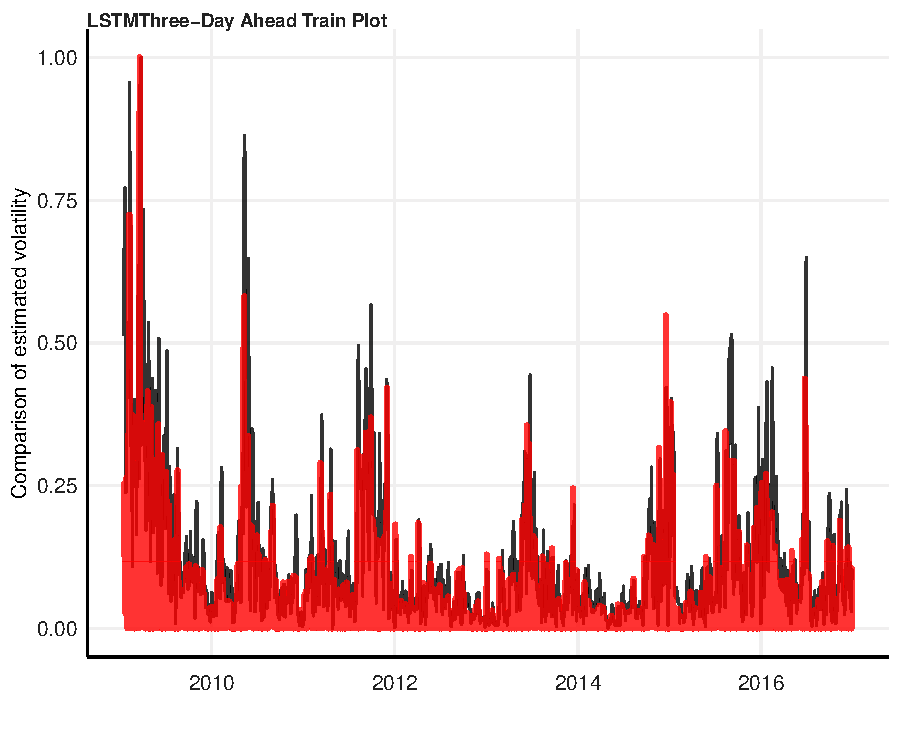
\includegraphics{Essay_files/figure-latex/plot_4-1} 

}

\caption{LSTM Three-Day Ahead Training Forecast}\label{fig:plot_4}
\end{figure}

\begin{figure}[H]

{\centering 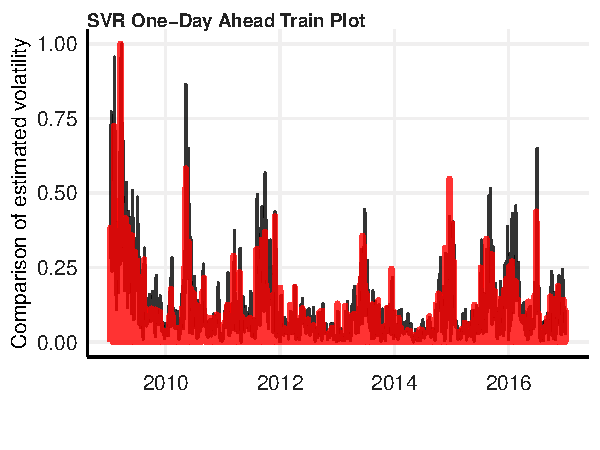
\includegraphics{Essay_files/figure-latex/plot_5-1} 

}

\caption{SVR One-Day Ahead Training Forecast}\label{fig:plot_5}
\end{figure}

\begin{figure}[H]

{\centering 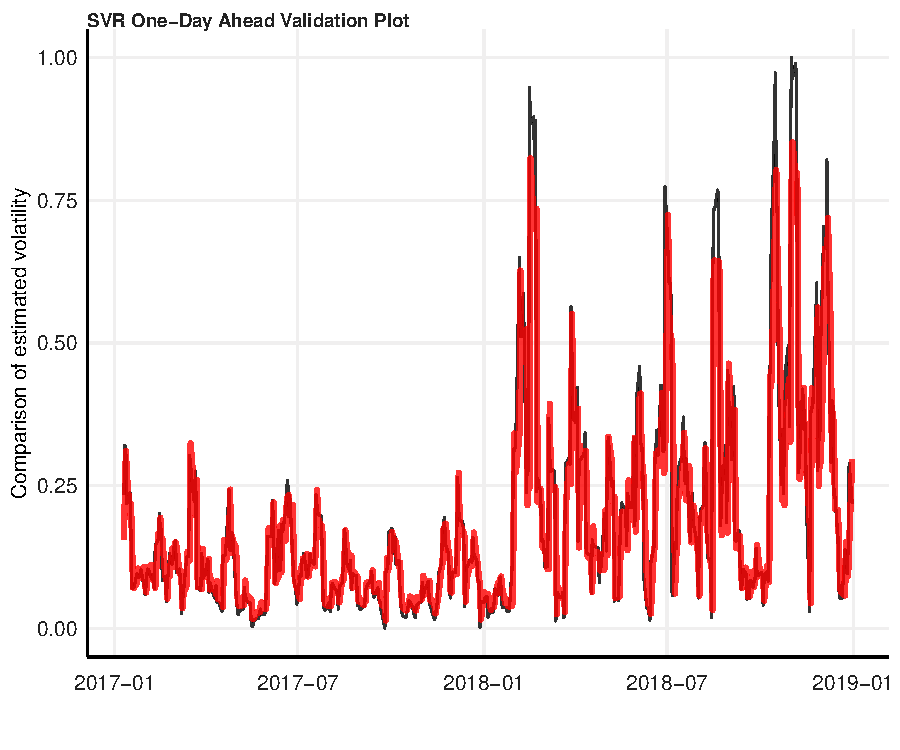
\includegraphics{Essay_files/figure-latex/plot_6-1} 

}

\caption{SVR One-Day Ahead Validation Forecast}\label{fig:plot_6}
\end{figure}

\begin{figure}[H]

{\centering 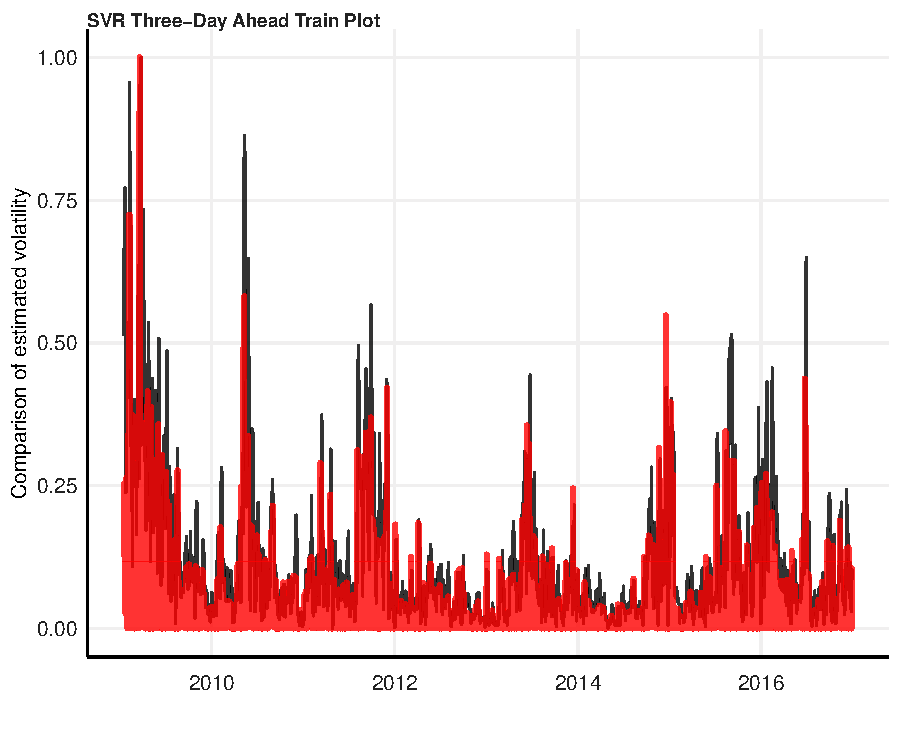
\includegraphics{Essay_files/figure-latex/plot_7-1} 

}

\caption{SVR Three-Day Ahead Training Forecast}\label{fig:plot_7}
\end{figure}

\begin{figure}[H]

{\centering 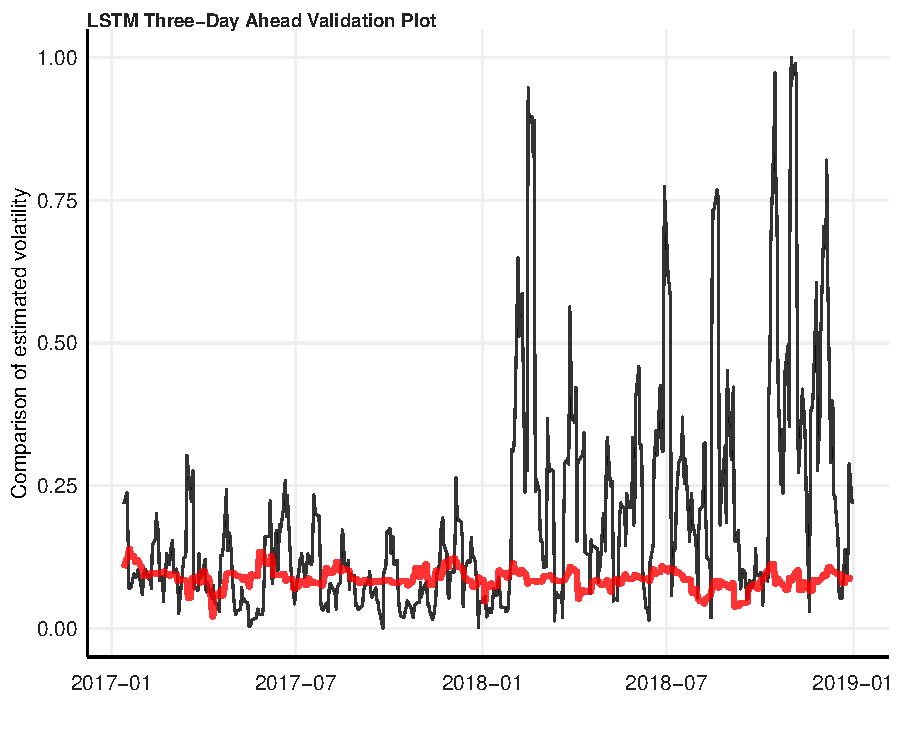
\includegraphics{Essay_files/figure-latex/plot_8-1} 

}

\caption{LSTM Three-Day Ahead Validation Forecast}\label{fig:plot_8}
\end{figure}

\begin{figure}[H]

{\centering 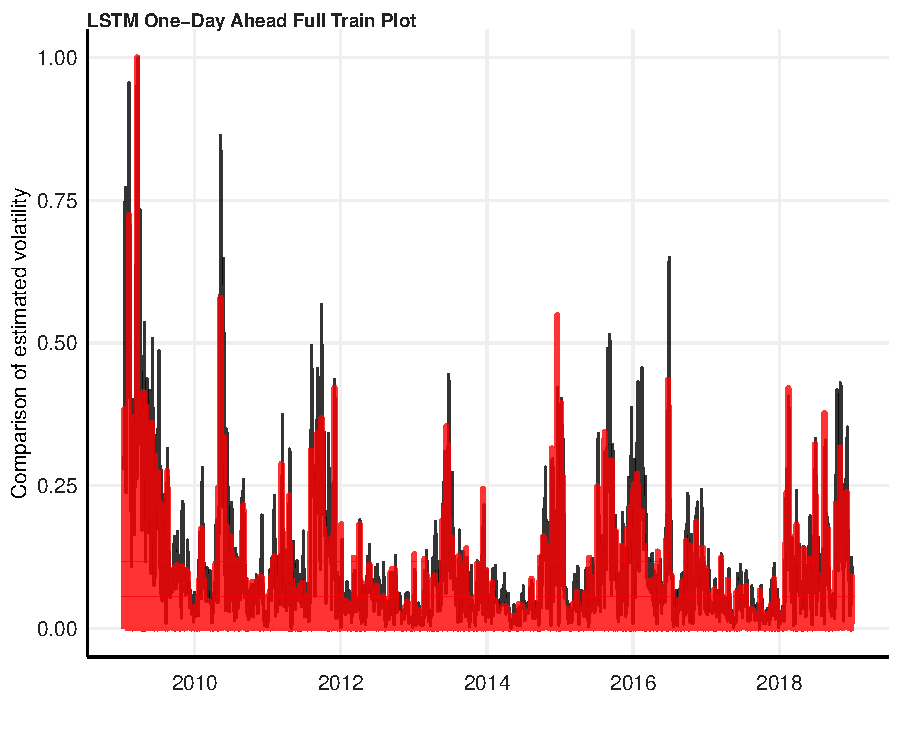
\includegraphics{Essay_files/figure-latex/plot_9-1} 

}

\caption{LSTM One-Day Ahead Full Training Forecast}\label{fig:plot_9}
\end{figure}

\begin{verbatim}
## NULL
\end{verbatim}

\bibliography{Tex/ref}





\end{document}
